\documentclass[12pt]{article}
\usepackage[utf8]{inputenc}
\usepackage{graphicx}
\usepackage{fullpage}
\usepackage{amsmath}
\usepackage{url}
\usepackage{float}
\usepackage{mathrsfs}
\usepackage{scalerel}
\usepackage{subcaption}


%----------------------------
\usepackage{here}
%\documentclass[11pt, english]{article}
%\usepackage{graphicx}
\usepackage[colorlinks=true, linkcolor=blue]{hyperref}
\usepackage[english]{babel}
\selectlanguage{english}
%\usepackage[utf8]{inputenc}
\usepackage[svgnames]{xcolor}
\usepackage{amssymb}
\usepackage{hyperref}
\usepackage{listings}
\usepackage{afterpage}
\pagestyle{plain}

\definecolor{dkgreen}{rgb}{0,0.6,0}
\definecolor{gray}{rgb}{0.5,0.5,0.5}
\definecolor{mauve}{rgb}{0.58,0,0.82}

%\lstset{language=R,
%    basicstyle=\small\ttfamily,
%   stringstyle=\color{DarkGreen},
%    otherkeywords={0,1,2,3,4,5,6,7,8,9},
%    morekeywords={TRUE,FALSE},
%    deletekeywords={data,frame,length,as,character},
%    keywordstyle=\color{blue},
%    commentstyle=\color{DarkGreen},
%}

\lstset{frame=tb,
language=R,
aboveskip=3mm,
belowskip=3mm,
showstringspaces=false,
columns=flexible,
numbers=none,
keywordstyle=\color{blue},
numberstyle=\tiny\color{gray},
commentstyle=\color{dkgreen},
stringstyle=\color{mauve},
breaklines=true,
breakatwhitespace=true,
tabsize=3
}




\textheight=21cm
\textwidth=17cm
%\topmargin=-1cm
\oddsidemargin=0cm
\parindent=0mm
\pagestyle{plain}

%%%%%%%%%%%%%%%%%%%%%%%%%%
% La siguiente instrucción pone el curso automáticamente%
%%%%%%%%%%%%%%%%%%%%%%%%%%

\usepackage{color}
\usepackage{ragged2e}

\global\let\date\relax
\newcounter{unomenos}
\setcounter{unomenos}{\number\year}
\addtocounter{unomenos}{-1}
\stepcounter{unomenos}
%\gdef\@date{ Course  2019}






%---------------------------


% \usepackage[lite]{mtpro2}
\title{\underline{Assignment 1} \\}
\author{Shreya Sharma}


\begin{document}
% \maketitle
%\vspace{7 cm}


\begin{center}
    
\vspace{1 cm}

\textbf{\Large{CS685: Data Mining} \\ \vspace{0.5 cm}\Large{Assignment 1} \\\vspace{0.5 cm}\Large{Shreya Sharma (19111087)}}\\
\vspace{1 cm} 
\end{center}
\section{Increment in Cases}
All the graph are generated from cases file. Cases in India are almost getting double with each passing month. Last month (Sept) have low number of cases as data is only upto 5th Sept. 2020. Weekly cases graph shows that there is no sign of convergence in the increment in the Covid cases and cases are increasing exponentially.
\begin{figure}[h!]
\centering
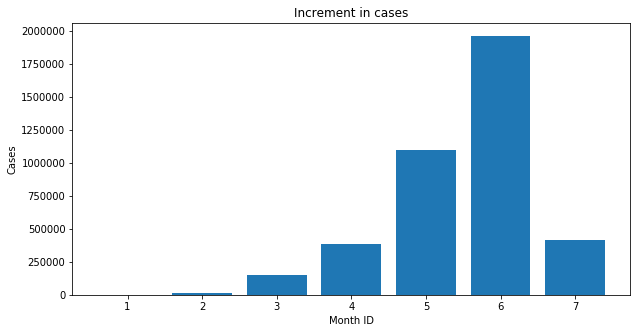
\includegraphics[scale=.4]{monthly-cases}
\caption{Monthly cases increment}
\end{figure}

\begin{figure}[h!]
\centering
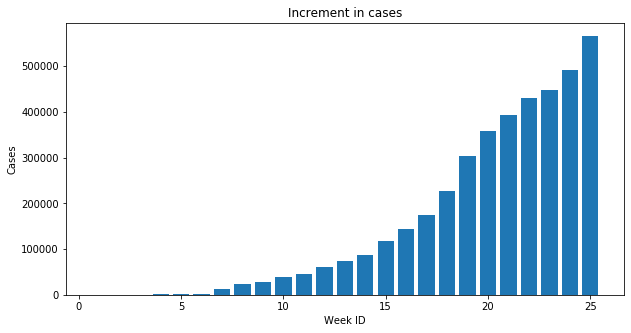
\includegraphics[scale=.4]{weekly-cases}
\caption{Weekly cases increment}
\end{figure}
\newpage
The graph below shows 50 percent of the cases in top 15 are from metropolitan cities like Pune, Delhi, Mumbai, Bengalore.  The below graph is interactive which can accessed using \href{https://top15withpect.html}{https://top15withpect.html} file present in Report folder. It also shows the number of cases of districts when hover over it.

\begin{figure}[h!]
\centering
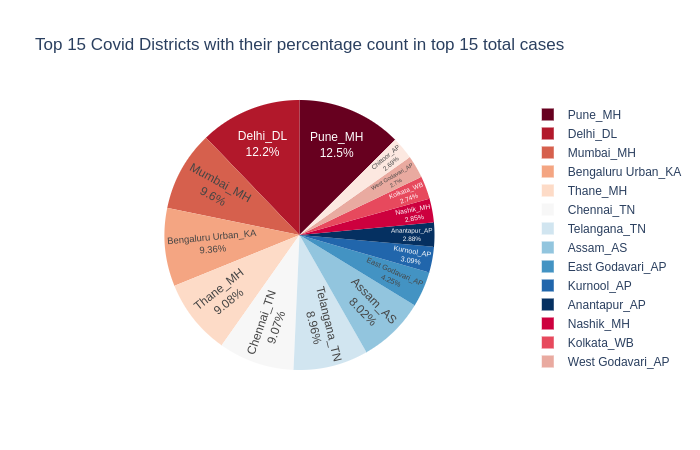
\includegraphics[scale=.5]{top15}
\caption{Top 15 districts with highest number of cases with their contribution in top-15}
\end{figure}
The below graph can be accessed using \href{https://top50.html}{https://top50.html} file present in Report folder. It shows that some of the districts are largely affected. After Assam (123k cases), there is large drop in number of cases in other districts like East godavari have only 65k cases.
\begin{figure}[h!]
\centering
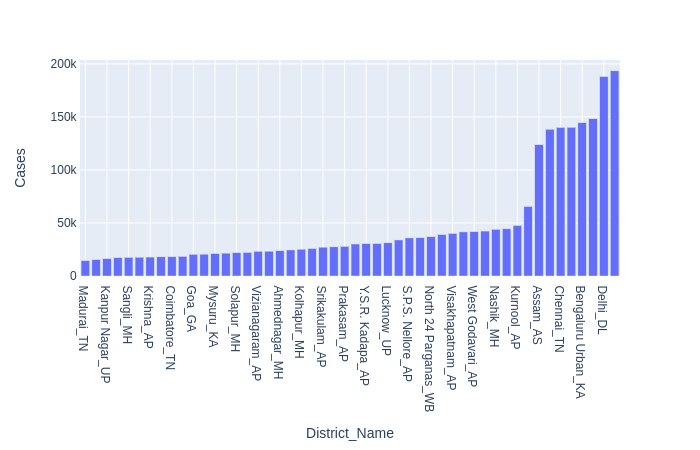
\includegraphics[scale=.4]{top50}
\caption{Most covid affected 50 districts}
\end{figure}
\newpage
The below graph can be accessed using \href{https://bottom50.html}{https://bottom50.html} file present in Report folder. States like Arunachal Pradesh, Mizoram, Meghalaya and Nagaland are least affected.
\begin{figure}[h!]
\centering
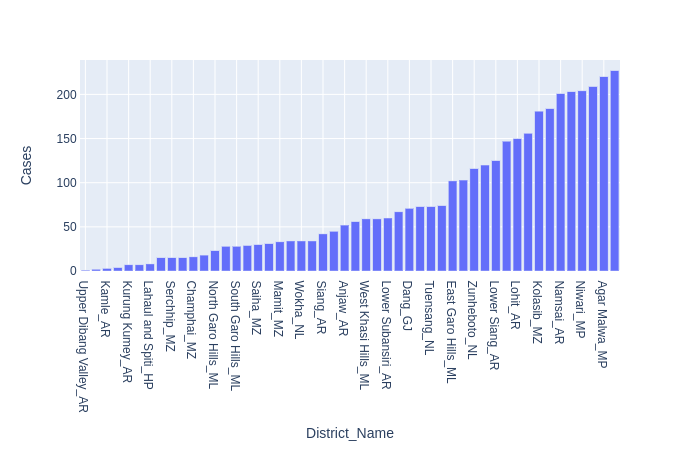
\includegraphics[scale=.6]{bottom50}
\caption{Least Covid affected 50 districts}
\end{figure}
\newpage

\section{Hotspot/Coldspot}
The below table stores the top 10 state wise hot and cold spot sorted by their occurences. It is calculated using method-spot-week.csv.\\
\\
\begin{tabular}{ |p{2cm}||p{14cm}|  }
 \hline
 \multicolumn{2}{|c|}{State wise hot/cold spot} \\
 \hline
 Monthly top 10 hotspot & Delhi, Assam, Telangana, Chandigarh, Bengaluru Urban, Rajkot, Jaipur, Ludhiana, Dehradun, Kota  \\
 \hline
 Monthly top 10 coldspot & Kodagu, Bhadohi, Diu, Charkhi Dadri, Jhargram, Kalimpong, Karaikal, Mahe, Sahibganj, Sheohar\\
 \hline
 Weekly top 10 hotspot & Delhi, Telangana, Assam, Vadodara, Indore, Surat, Bhopal, Chennai, Bengaluru Urban, Jabalpur  \\
 \hline
 Weekly top 10 coldspot & Diu, Mahe, Perambalur, Karaikal, Sheohar, Porbandar, Kalimpong, Bhadohi, Jhargram,
 Agar Malwa\\
 \hline
\end{tabular}\\ \\
\\
The graph below shows the number of hotspot occuring in a week. The graph is generated using method-spot-week.csv. It shows that now the increment in number of hotspot are now stable.
\begin{figure}[h!]
\centering
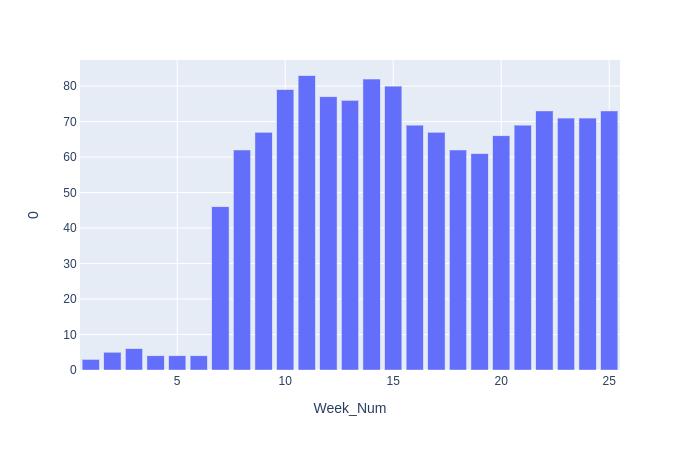
\includegraphics[scale=.5]{newplot (5).png}
\caption{Weekly state hotspot increment}
\end{figure}
\newpage
The graph below shows the number of hotspot occuring in a week considering neighbors. Neighbor hotspots are more than state hotspots. The graph is generated using method-spot-week.csv. It shows that now the increment in number of hotspot are stable. 
\begin{figure}[h!]
\centering
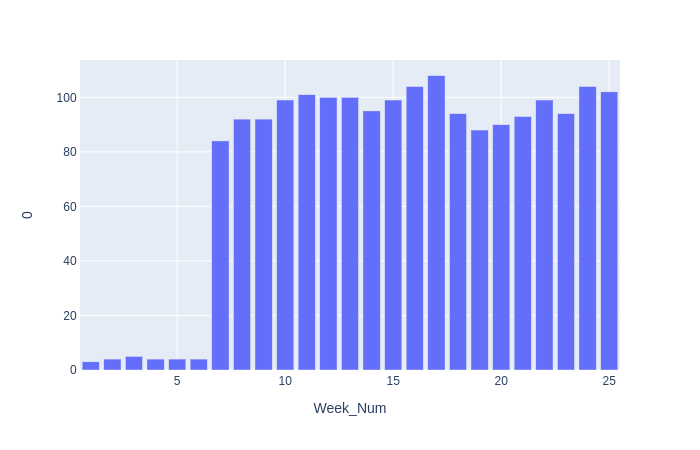
\includegraphics[scale=.7]{newplot (7).png}
\caption{Weekly neighborhood hotspot increment}
\end{figure}
\end{document}